%!TEX root = ../../fourthYearReport.tex

\paragraph{Work package 5 progress}

The activities in WP5 are divided into four tasks corresponding to the four years project duration. As a result, during the fourth year CoDyCo results concentrate on T5.4. The main result consist in the implementation of the validation scenario consisting of the balancing with the help of a caregiver. The main scientific contribution is described here \cite{latella2016whole}.

\subparagraph{Scenario 4: learning how to stand up with the help of a human caregiver (T5.4)}

The main contributions to T5.4 have been presented in ``Validation scenario 4: learning how to stand up with the help of a human caregiver'' which discusses the technical implementation of the fourth year validation scenario (see \url{https://github.com/robotology-playground/codyco-deliverables/tree/master/D5.4/pdf}). The software developed for the scenario implementation is released with an open-source license and distributed through github (\url{https://github.com/robotology/codyco}).


\textbf{CoM Dynamic Manipulability for the iCub in a Sitting Configuration}


In this calculations, it is assumed that the robot is in a sitting
configuration with joint angles mentioned in Table \ref{jointangles}.
Shoulder pitch angle ($\alpha$) and elbow angle ($\beta$) are the two
variables which are used to maximize the CoM dynamic manipulability in a
desired direction.  The desired direction of the CoM movement in the beginning
of the motion is horizontal.  The maximum joint torques are assumed to be
$40$N.m. for the legs and $20$N.m. for the arms.
%
\begin{table}[h]
  \centering
  \caption{iCub joint angles in a sitting configuration.  Angles are in
    degrees.}
  \begin{tabular}{|c|c||c|c||c|c|}
    \hline hip pitch   & $91$   & shoulder roll & $12$ & torso pitch & $-5$ \\
    \hline hip roll    & $12$   & shoulder yaw  & $80$ & torso roll  & $0$   \\
    \hline hip yaw     & $0$    & wrist pronos  & $0$  & torso yaw   & $0$   \\
    \hline knee        & $-104$ & wrist pitch   & $0$  & neck pitch  & $0$ \\
    \hline ankle pitch & $-12$  & wrist yaw     & $0$  & neck roll   & $0$ \\
    \hline ankle roll  & $0$    &               &      & neck yaw    & $0.5$ \\
    \hline
  \end{tabular}
  \label{jointangles}
\end{table}
%
\begin{figure}
  \centering
  \includegraphics[scale=0.29]{3Dfigure.pdf}
  \caption{CoM dynamic manipulability with respect to arm configuration.}
  \label{3Dfig}
\end{figure}
%


The CoM dynamic manipulability for different arm configurations
(i.e. different $\alpha$ and $\beta$) is shown in Figure \ref{3Dfig}.  The
maximum manipulability is at $\alpha = -29^\circ$ and $\beta = 32^\circ$.
Figures \ref{2Dfig_shoulder} and \ref{2Dfig_elbow} show CoM manipulability
with respect to the shoulder angle and the elbow angle, respectively.  As it
can be seen in these figures, in case the optimum values are not feasible,
best values for the shoulder angle value is between $-20^\circ$ to $-40^\circ$
and for the elbow angle is about $30^\circ$.  Figures \ref{icub_optimum} shows
the iCub's configurations when the arms angles are in their optimum values.
Figrue \ref{icub_suboptimum} shows the iCub's configuration when $\alpha =
-40^\circ$ and $\beta = 32^\circ$.  In this case, the manipulability is
decreased by $\%3$.
%
\begin{figure}
  \centering \includegraphics[scale=0.4]{2DfigureShoulder.pdf}
  \caption{CoM dynamic manipulability with respect to shoulder pitch angle.}
  \label{2Dfig_shoulder}
\end{figure}
%
\begin{figure}
  \centering
  \includegraphics[scale=0.4]{2DfigureElbow.pdf}
  \caption{CoM dynamic manipulability with respect to elbow angle.}
  \label{2Dfig_elbow}
\end{figure}
%
\begin{figure}
  \centering 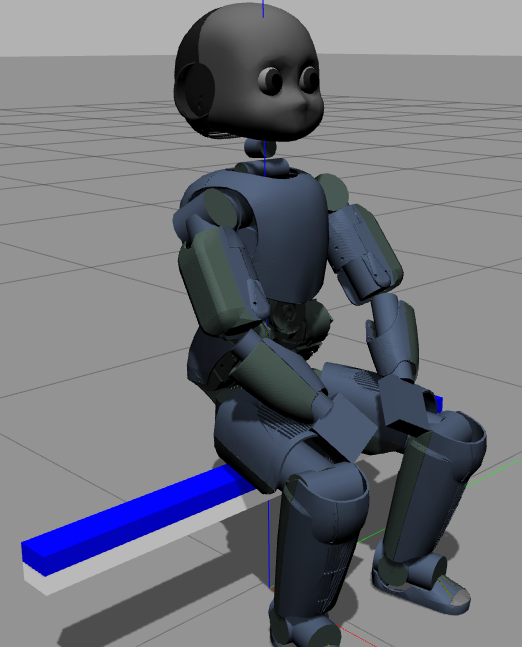
\includegraphics[scale=0.4]{icub_optimum}
  \caption{iCub in optimum sitting configuration.}
  \label{icub_optimum}
\end{figure}
%
\begin{figure}
  \centering
  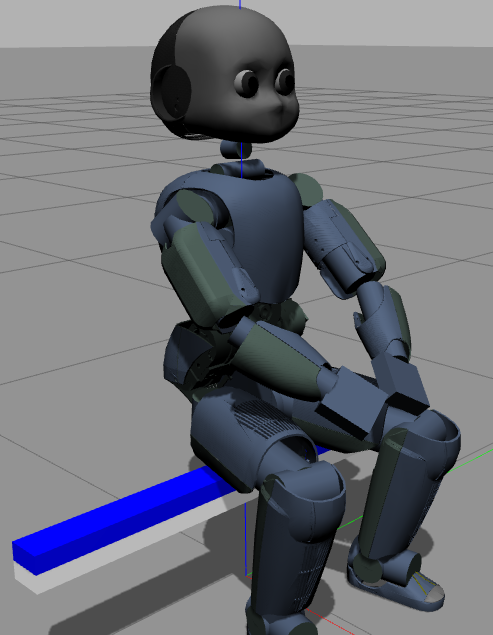
\includegraphics[scale=0.4]{icub_suboptimum}
  \caption{iCub in near-optimum sitting configuration.}
  \label{icub_suboptimum}
\end{figure}
%



\subparagraph{Deviations from workplan}  

No deviations.

%\begin{itemize}
%\item[-] \emph{\color{red}[A summary of progress towards objectives and details for each task;]}
%\item[-] \emph{\color{red}[Highlight clearly significant results;]}
%\item[-] \emph{\color{red}[If applicable, explain the reasons for deviations from Annex I and their impact on other tasks as well as on available resources and planning;]}
%\item[-] \emph{\color{red}[If applicable, explain the reasons for failing to achieve critical objectives and/or not being on schedule and explain the impact on other tasks as well as on available resources and planning (the explanations should be consistent with the declaration by the project coordinator) ;]}
%\item[-] \emph{\color{red}[a statement on the use of resources, in particular highlighting and explaining deviations between actual and planned  person-months per work package and per beneficiary in Annex 1 (Description of Work);]}
%\item[-] \emph{\color{red}[If applicable, propose corrective actions.]}
%\end{itemize}
